% HRI Pioneers 2027 -- anonymous extended abstract.
% Limits: 2 pages + up to 1 page of references; abstract ~100-150 words.
% Anonymisation (Pioneers rule): describe own prior work in first person, but
% anonymise those entries in the reference list (see references.bib).
\documentclass[sigconf,review,anonymous,nonacm]{acmart}
\setcopyright{none}
\settopmatter{printacmref=false}
\acmConference[HRI '27]{ACM/IEEE International Conference on Human-Robot Interaction}{2027}{}

\begin{document}
\raggedbottom
\title{When, Where, and Whether to Speak: Training Robots to Communicate as Teammates}

\begin{abstract}
Large Language Models (LLMs) have made robots fluent in \emph{what} to say. Natural collaboration, however, demands knowing \emph{when} to speak, \emph{where} to direct attention, and \emph{whether} to act at all, skills humans master and machines still lack. Unlike text, interaction datasets are scarce, and the cues that matter are spread across modalities. My research asks how LLM-based agents can acquire these skills, matching each adaptation to the data available for it. I built a collaborative-game testbed and corpus, and models that turn interaction data into supervision signals, from self-reported enjoyment to brain activity. I now adapt an open full-duplex Spoken Language Model to decide in real time, fine-tuning it where data is abundant (self-play, gaze) and steering it with lightweight interventions where data is scarce (human signals). My aim is robots that take part in shared tasks as helpful teammates, adapting to each partner rather than expecting the opposite.
\end{abstract}

\begin{CCSXML}
<ccs2012>
 <concept><concept_id>10003120.10003121</concept_id><concept_desc>Human-centered computing~Human computer interaction (HCI)</concept_desc><concept_significance>500</concept_significance></concept>
 <concept><concept_id>10010147.10010178.10010179</concept_id><concept_desc>Computing methodologies~Natural language processing</concept_desc><concept_significance>300</concept_significance></concept>
</ccs2012>
\end{CCSXML}
\ccsdesc[500]{Human-centered computing~Human computer interaction (HCI)}
\ccsdesc[300]{Computing methodologies~Natural language processing}
\keywords{Human--robot collaboration, full-duplex dialogue, turn-taking, gaze, model steering, data efficiency}

\begin{teaserfigure}
 \centering
 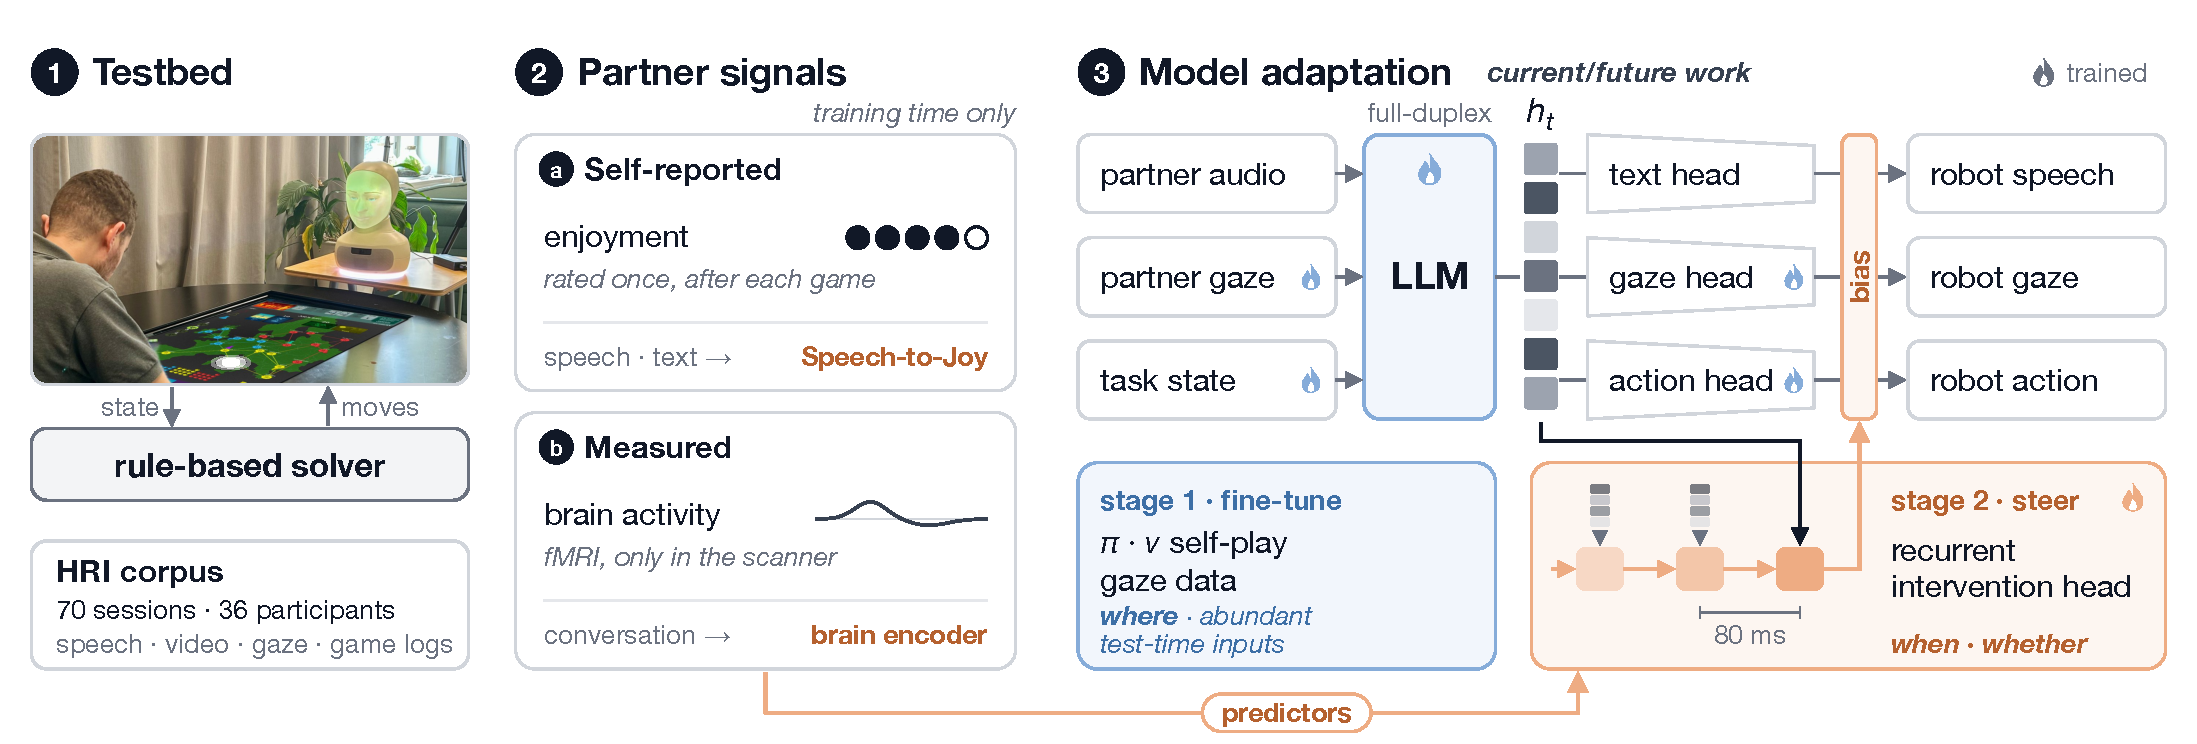
\includegraphics[width=\textwidth]{figures/header.pdf}
 \caption{Research overview, in PhD order. (1)~Testbed: a participant and a Furhat robot play \emph{Pandemic}; a rule-based solver plays the robot's side and grounds pre-scripted and generated dialogue conditions. (2)~Supervision signals (a)~derived from the resulting corpus. (b) and (c)~collected from multiple open HRI datasets. (3)~Model adaptation: a full-duplex model hears the partner, sees their gaze and reads the task state, and every 80\,ms decides whether to speak, act, or where to look. Stage~1 (blue) fine-tunes it where data is abundant. Stage~2 (orange) freezes it and trains a recurrent intervention head over its hidden states $h_t$ that biases its logits, supervised by the signals of (2).}
 \Description{Three columns in one row, ordered in time, with no arrows between columns. Column 1, Testbed: photo of a participant at a touchscreen table with a game map, a Furhat robot head opposite; below it, arrows labelled state and moves connect the photo to a grey block labelled rule-based solver; below that, a box labelled HRI corpus, 70 sessions, 36 participants, speech, video, gaze and game logs. Column 2, Supervision: three equal boxes. Observed lists speech with a waveform, video with a film strip, and game state. Self-reported lists engagement, enjoyment and cognitive effort, each with a row of five small rating dots. Measured lists brain activation with a haemodynamic response curve, eye tracking, and task performance marked win. Column 3, Model adaptation, tagged current/future work: partner audio, partner gaze and task state feed a pale blue LLM labelled full-duplex and marked trained, whose hidden state h_t feeds white trapezoidal text, gaze and action heads; partner gaze, task state, gaze head and action head carry small blue flames, marking them as trained in stage 1; their outputs pass through a pale peach bias block to robot speech, robot gaze and robot action. Below, two boxes of equal height. A pale blue box labelled stage 1, fine-tune, lists pi and v self-play and gaze data, labelled abundant task plus conversational data. A pale peach box labelled stage 2, steer, recurrent intervention head, and scarce signals (2), shows three recurrent cells unrolled over 80 ms frames, each receiving a hidden state, the last one h_t from the LLM; the last cell drives the bias. A legend reads: flame, trained.}
 \label{fig:overview}
\end{teaserfigure}
\maketitle

\section{Introduction}

Large Language Models (LLMs) have made robots fluent in \emph{what} to say. Turning robots from tools into teammates that augment rather than replace people~\cite{akata2020research} also requires knowing \emph{when} to speak or act, \emph{where} to direct attention in the shared space, and \emph{whether} to act at all given the partner's state. People regulate these with timing, gaze, and the state of the shared task~\cite{skantze2021turn}, cues that LLM-based agents neither perceive nor produce.

The data for these skills is not equally available. Task data is effectively unlimited, since a game engine can generate self-play indefinitely~\cite{silver2018alphazero}. Conversational gaze follows regularities that hold across settings~\cite{skantze2021turn}, so it can be learned from large corpora of human interaction~\cite{agrawal2025seamless}. However, the signals that say whether an interaction worked for \emph{this} partner are scarce and spread across modalities: Our corpus, for instance, spans 70 sessions with 36 participants~\cite{anon2026dataset}. I therefore match each adaptation to the data available for it, fine-tuning a full-duplex model where data is abundant and \emph{steering} it, through a small learned intervention on the frozen model, where it is scarce (Fig.~\ref{fig:overview}).
\begin{itemize}
 \item \textbf{RQ1 (\emph{when and whether}):} Can a full-duplex model be steered, from one study's data, to take turns and act at human-like moments?
 \item \textbf{RQ2 (\emph{where}):} How can task state and gaze, as input and output, ground dialogue in the shared task space?
 \item \textbf{RQ3 (\emph{how}):} Which human signals (observed, self-reported, measured) can be predicted from interaction data, and can these predictions supervise model adaptation?
\end{itemize}

\section{Background}

\paragraph{Coordinating turns, gaze, and initiative}
People exchange turns with gaps of around 200\,ms. Skantze~\cite{skantze2021turn} reviews the cues behind this projection, from syntax and prosody to gaze and the state of a shared task. Predictive models learn it from data, TurnGPT~\cite{ekstedt2020turngpt} from text and Voice Activity Projection (VAP)~\cite{ekstedt2022vap} from dyadic audio, and VAP has reduced delays and interruptions on an LLM-driven Furhat~\cite{skantze2025applying}. Gaze regulates the floor~\cite{admoni2017social} and directs joint attention, and a robot whose gaze responds to its partner's is rated as more socially present~\cite{pereira2019responsive}. TurnGPT and VAP predict when the floor opens, not whether there is reason to take it~\cite{peng2026full}.

\paragraph{Real-time grounding}
Real-time multimodal LLMs can steer a robot's gaze through tool calls, but they decide once per turn and often miss when to look~\cite{lee2026recipe}. Open full-duplex models~\cite{defossez2024moshi,roy2026personaplex} decide every 80\,ms frame, as tokens, and are gaining channels beyond speech: tool calls co-decoded with speech on one clock~\cite{zhang2026duplexsla, balam2026nemotronlabsvoicechatopenfullduplex}, and facial motion generated alongside it~\cite{jiang2026moshiface}. Yet they speak when addressed or at silence, and even when handed the floor they rarely correct a false claim or warn of a hazard~\cite{peng2026full}. Game agents ground their communication in a policy-value network~\cite{kramar2022negotiation,bakhtin2022cicero}, and projecting an engine's hidden state into an LLM as tokens outperforms describing it in text~\cite{si2026exploring}. I bring this to full duplex, adding task state and partner gaze as input streams and robot gaze as an output channel.

\paragraph{Adapting from scarce human signals}
Human signals are too costly to supervise training directly, so Reinforcement Learning from Human Feedback (RLHF) fits a reward model to them and optimizes against it instead~\cite{christiano2017deep,ouyang2022rlhf}. Whether an interaction worked for \emph{this} partner is scarcer still, yet predictable from interaction data, from self-reported and annotated enjoyment~\cite{pereira2024multimodal,anon2025joy} to the conversational partner's brain responses~\cite{zada2026linguistic,anon2026fmri}. Such predictors could supervise adaptation, which leaves where to intervene. Context (through prompts) shapes \emph{what} is said more than \emph{when}, and weight updates~\cite{hu2022lora,rafailov2023dpo} need more data than HRI provides. Activation steering~\cite{turner2023actadd,rimsky2024caa,zou2023repe} is data-efficient and corrects slow yielding in full-duplex models~\cite{chang2026overcoming}, but can also shift content, whereas logit steering~\cite{yang2021fudge,krause2021gedi} reweights only the next token.

\section{Prior Work: Testbed and Supervision}

\paragraph{Testbed and observed behaviour}
I co-developed an open platform in which a participant and a Furhat robot~\cite{al2012furhat} play the cooperative board game \emph{Pandemic} on a shared touchscreen, with an inspectable game engine, a rule-based solver playing the robot's side, and LLM-based grounded dialogue system~\cite{anon2026platform}. With it, a corpus 70 interactions with 36 participants was collected, each playing once with a game-adaptive and once with a generic robot voice: diarized transcripts annotated for interaction failures, isolated participant and robot audio, facial action units, head pose and classified gaze, aligned with game states, robot logs, and questionnaires~\cite{anon2026dataset}. This is the \emph{observed} reference steering should match (part~2a).

\paragraph{Self-reported experience}
Self-reports are ground truth for experience but arrive once, afterwards. Speech-to-Joy predicts post-interaction enjoyment from frozen speech and text embeddings, correlating with self-reports more strongly than an experienced HRI annotator and LLM baselines, even from audio alone, and is light enough for real-time use~\cite{anon2025joy}. My corpus includes per-game enjoyment ratings, so the predictor can be retrained there as a proxy for a self-reported objective (part~2b).

\paragraph{Measured signals}
I adapted a multimodal whole-brain fMRI foundation model to live conversation, improving held-out prediction by 15\% over a ridge encoder~\cite{anon2026brainconv}. Across two conversational fMRI corpora with human and robot partners (70 participants), transfer between partners was asymmetric where the robot's visual behaviour differed most from a human's, and corpus differences mattered more than partner identity~\cite{anon2026brainhri}. Gaze and task performance, logged in my corpus, complete the measured signals (part~2c).

\section{Current and Future Work: Model Adaptation}
\label{sec:current}

\paragraph{Steering when to act (RQ1, pilot)}
Off the shelf, the model proposed 3.5$\times$ as many speech onsets as the participant it replaced, yet matched only a quarter of theirs ($\pm$960\,ms). Prompt rewrites did not change when it acted, and vetoes after the argmax failed: the model re-proposed, and denying every proposal silenced it for good. Interventions before the argmax worked, and the hidden state appears to know more than the head: a small recurrent head over $h_t$ predicted the partner's next onset with AUC 0.87 (leave-one-participant-out, 18 participants, under 400 onsets), against 0.51 for the model's own start-versus-wait margin, doubling onset recall at the same false-start rate. One study's data may thus suffice to read the state; whether steering on it improves interaction needs closed-loop evaluation, which comes next.

\paragraph{Stage 1: task and gaze channels (RQ2)}
The second pilot asks whether self-play can supply task state worth injecting. On a JAX port of the game, a policy--value network trained by imitation and then Gumbel AlphaZero self-play~\cite{silver2018alphazero,danihelka2022gumbel} wins 71\% of games at rulebook difficulty, against 24\% for the solver. Its last hidden layer is one candidate for the task-state stream. For gaze, I plan to add partner gaze as input and a head emitting quantised gaze tokens alongside speech~\cite{jiang2026moshiface,mentzer2024fsq}. In the corpus, the robot looking at the participant predicts their next onset a second ahead, suggesting gaze is a turn-yielding lever the robot controls. After fine-tuning, the steering head is retrained to steer gaze as well as speech.

\paragraph{Stage 2: closing the loop (RQ3)}
The head so far matches \emph{observed} behaviour. I will supervise it with predicted \emph{self-reported} and \emph{measured} signals, either as targets that calibrate the bias per partner and moment, or as rewards for a low-dimensional policy over a few logits, learned with contextual bandits offline on the corpus and then online. The override failures set a safety constraint: bias, but never deny every turn.

\section{Conclusion}
For a robot teammate, collaboration and adaptation start with timing: knowing when to speak, where to look, and whether to act, and tuning all three to the partner at hand. My recipe fine-tunes open full-duplex models where data is abundant and steers them with what a single study yields.

\clearpage
\balance
\bibliographystyle{ACM-Reference-Format}
\bibliography{references}
\end{document}
